\subsubsection{Dịch vụ văn bản (document service)}

Sơ đồ tổng quan về dịch vụ văn bản (Document Service):

\begin{figure}[H]
\centering
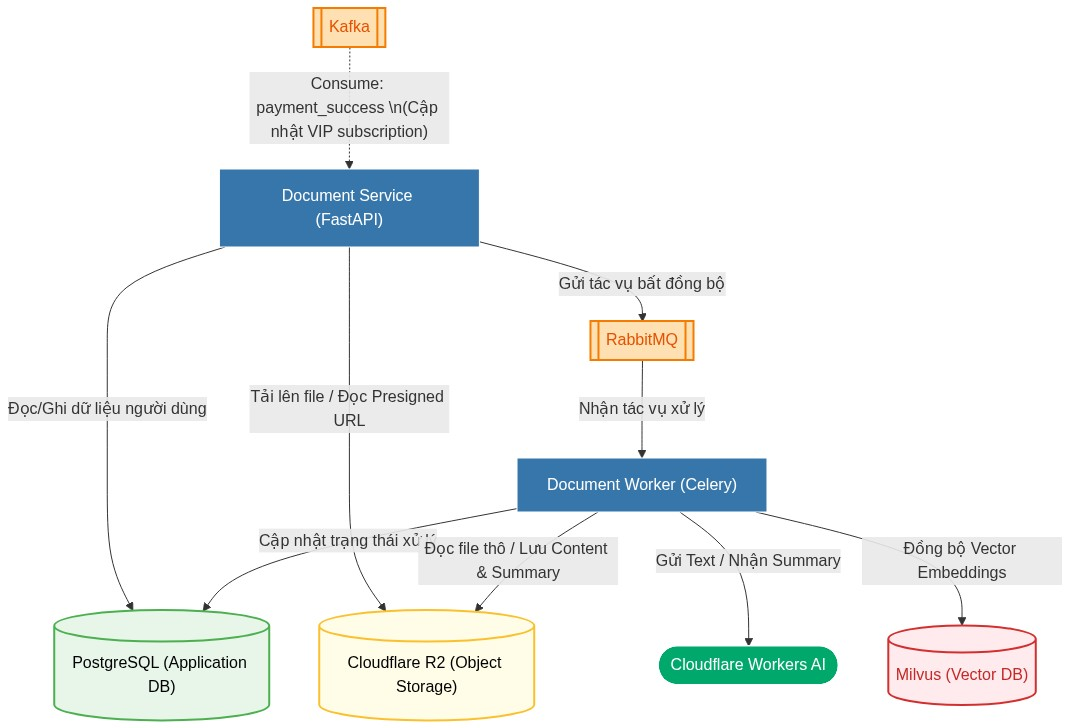
\includegraphics[width=0.99\textwidth]{pictures/document-overview.png}
\caption{Sơ đồ tổng quan dịch vụ văn bản}
\end{figure}

% Mục đích:
Tiếp nhận, lưu trữ và quản lý luồng xử lý tài liệu của người dùng. Dịch vụ này không chỉ lưu trữ tệp tin mà còn hỗ trợ quy trình trích xuất nội dung sang định dạng Markdown, tự động tạo bản tóm tắt và thực hiện vector hóa tài liệu.

\begin{figure}[H]
\centering
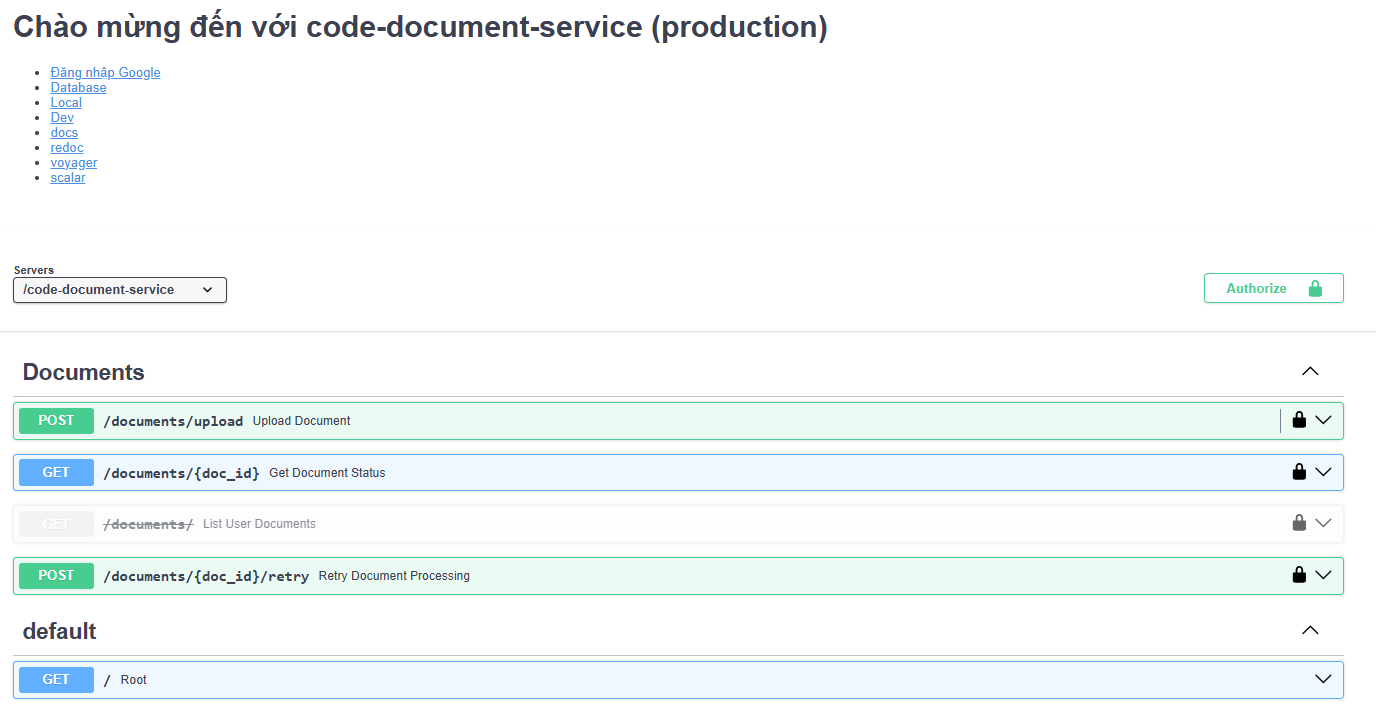
\includegraphics[width=0.95\textwidth]{pictures/document-swagger.png}
\caption{Tài liệu Swagger API dịch vụ văn bản}
\end{figure}

Vì chức năng tải lên tài liệu chỉ dành riêng cho người dùng sở hữu gói VIP, dịch vụ văn bản (Document Service) thực hiện lắng nghe sự kiện thanh toán thành công từ Kafka, lưu thông tin vào CSDL để kiểm tra và xác thực quyền VIP của người dùng hiện tại.

\begin{itemize}
\item \textbf{Tải lên tài liệu mới}: Người dùng gửi tệp tài liệu lên hệ thống. Sau khi tiếp nhận thành công, hệ thống sẽ trả về mã định danh duy nhất (\texttt{doc\_id}), tên tệp gốc và trạng thái khởi tạo ban đầu, đồng thời đưa tác vụ vào hàng đợi xử lý.

\item \textbf{Truy xuất trạng thái xử lý}: Dựa vào \texttt{doc\_id}, người dùng có thể truy vấn trạng thái xử lý hiện tại của tài liệu. Hệ thống sẽ báo cáo chi tiết về sự tồn tại của các thành phần dữ liệu thông qua các cờ trạng thái: \texttt{has\_file}, \texttt{has\_content}, \texttt{has\_summary}.

\item \textbf{Thử lại tác vụ lỗi}: Trong trường hợp quá trình bóc tách hoặc tóm tắt gặp sự cố, hệ thống cung cấp một API chuyên biệt để kích hoạt lại quy trình xử lý cho tài liệu đó mà không cần người dùng phải tải lên lại tệp gốc.
\end{itemize}

\paragraph{Document Worker}

Dịch vụ văn bản kết hợp với \textbf{Document Worker} (nhận các tác vụ nền từ Celery thông qua RabbitMQ) để thực hiện quy trình xử lý tài liệu phục vụ hệ thống RAG:

\begin{enumerate}
\item \textbf{Tải tệp tin}: Tải tệp tin từ Cloudflare R2 và sử dụng thư viện \texttt{Docling} để bóc tách cấu trúc và nội dung văn bản.
\item \textbf{Tóm tắt văn bản}: Sử dụng mô hình ngôn ngữ trên Cloudflare Workers AI để tự động tạo bản tóm tắt nội dung tài liệu bằng tiếng Việt.
\item \textbf{Chia nhỏ văn bản (Chunking)}: Sử dụng bộ chia \texttt{RecursiveCharacterTextSplitter} của LangChain để chia nhỏ văn bản thành các đoạn phù hợp.
\item \textbf{Trích xuất đặc trưng (Embedding)}: Tạo vector biểu diễn ngữ nghĩa cho từng đoạn văn bản bằng mô hình \texttt{keepitreal/vietnamese-sbert}.
\item \textbf{Lưu trữ Vector}: Quản lý và lưu trữ các vector embedding vào CSDL vector Milvus để phục vụ tìm kiếm ngữ nghĩa sau này.
\end{enumerate}

\paragraph{Cơ chế tối ưu \& Độ bền bỉ (Optimization \& Resilience)}

\begin{itemize}
\item \textbf{Tái sử dụng kết quả (Deduplication)}: Để tối ưu chi phí và hiệu năng, trước khi chạy parser và AI, worker kiểm tra xem người dùng đã từng tải lên tệp tin có cùng dung lượng (\texttt{file\_size}) và băm (\texttt{file\_hash}) hay chưa. Nếu đã có tài liệu trùng khớp đã xử lý thành công, hệ thống sao chép trực tiếp kết quả bóc tách và tóm tắt trên Cloudflare R2 sang đường dẫn của tài liệu mới mà không cần chạy lại mô hình AI.

\item \textbf{Cấu hình hàng đợi Celery bền bỉ}: Thiết lập \texttt{task\_acks\_late=True} để task chỉ được xóa khỏi RabbitMQ khi worker đã hoàn thành thực tế (tránh mất mát tác vụ), thiết lập \texttt{worker\_prefetch\_multiplier=1} ép worker chỉ nhận 1 tài liệu tại một thời điểm để cân bằng tả, tự động thử lại tối đa 3 lần (mỗi lần chờ 60 giây) nếu gặp sự cố kết nối.

\item \textbf{Giám sát Langfuse}: Toàn bộ luồng tóm tắt văn bản bằng AI (Cloudflare Workers AI) được theo dõi vết và giám sát chi tiết thông qua nền tảng \textbf{Langfuse} để kiểm soát chất lượng và độ trễ.
\end{itemize}

Giao diện quản lý vector trên Milvus:

\begin{figure}[H]
\centering
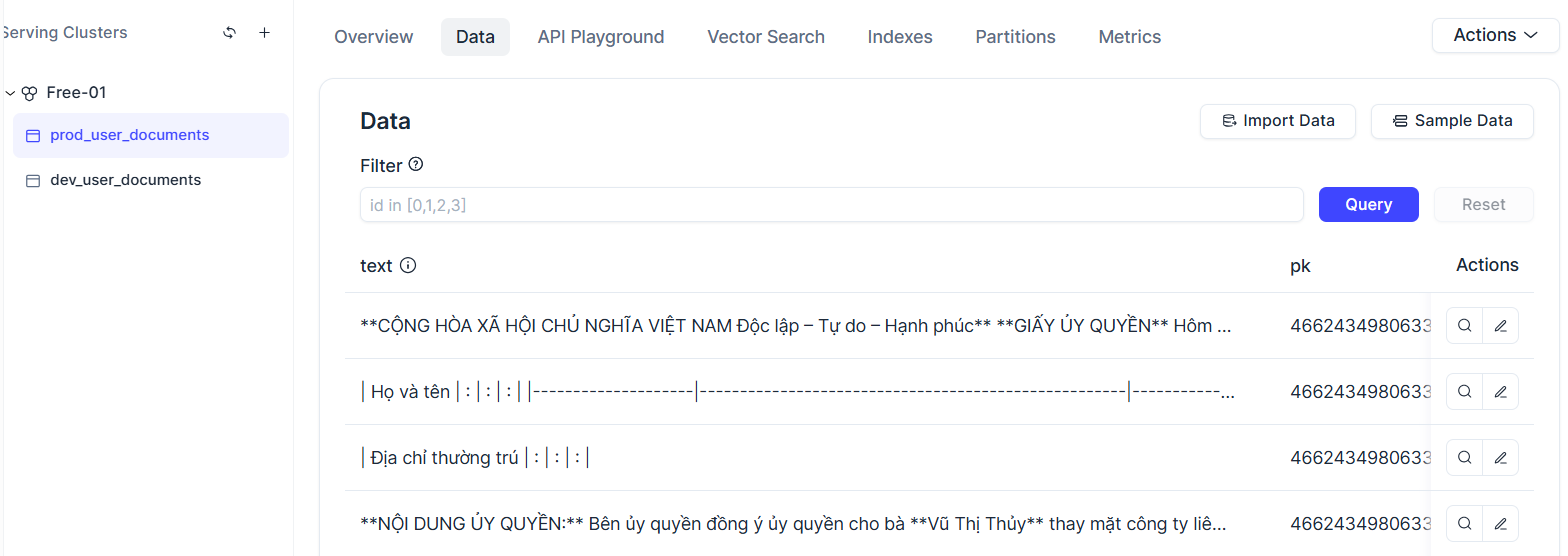
\includegraphics[width=0.99\textwidth]{pictures/document-milvus.png}
\caption{Dữ liệu vector lưu trữ trên Milvus}
\end{figure}

Quản lý các file tài liệu gốc trên Cloudflare R2:

\begin{figure}[H]
\centering
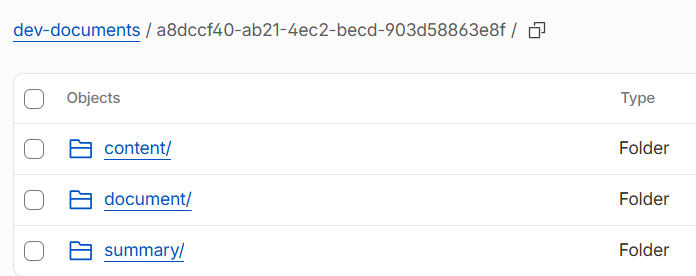
\includegraphics[width=0.85\textwidth]{pictures/r233333.png}
\caption{Kết quả lưu trữ tài liệu trên Cloudflare R2}
\end{figure}

Quản lý nội dung tóm tắt lưu trữ trên Cloudflare R2:

\begin{figure}[H]
\centering
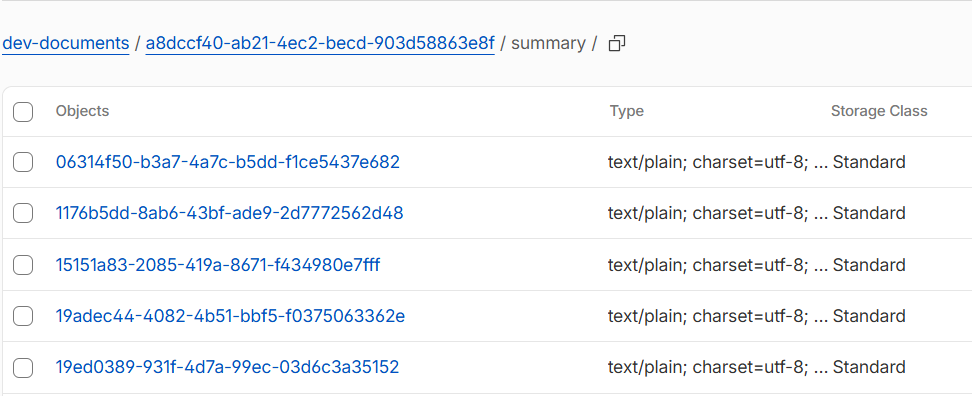
\includegraphics[width=0.85\textwidth]{pictures/r2summmmmm.png}
\caption{Bản tóm tắt lưu trữ trên Cloudflare R2}
\end{figure}

Quản lý di chuyển CSDL của dịch vụ văn bản:

\begin{figure}[H]
\centering
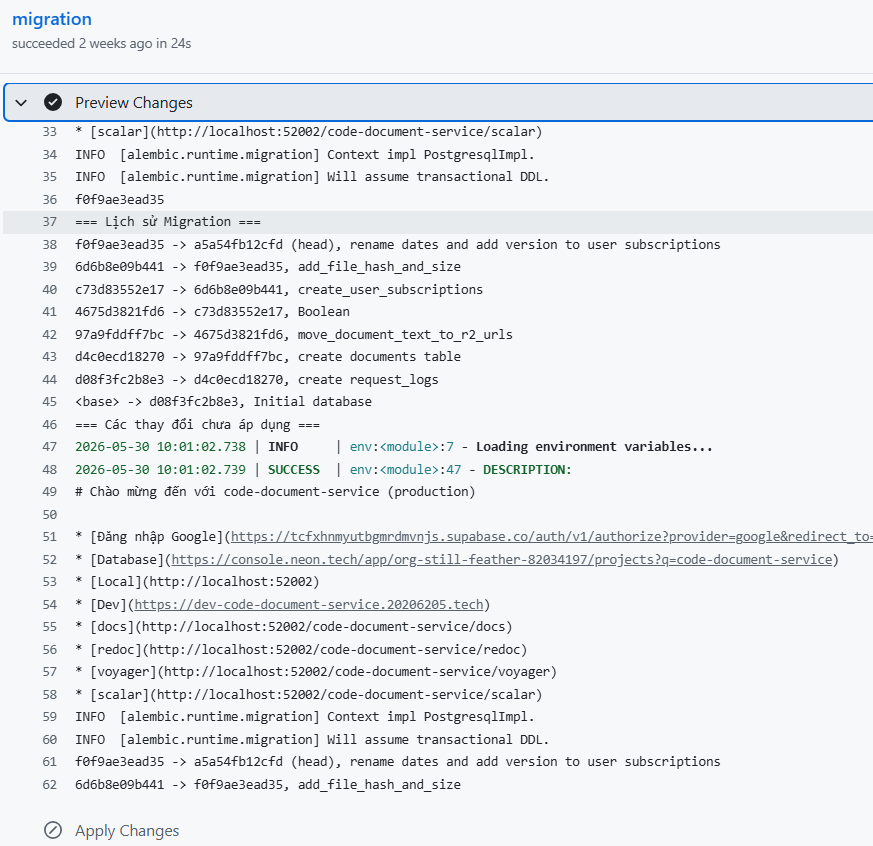
\includegraphics[width=0.7\textwidth]{pictures/document-database-migration.png}
\caption{Quản lý di chuyển CSDL của dịch vụ văn bản}
\end{figure}

Kết quả các bảng trong CSDL tài liệu:

\begin{figure}[H]
\centering
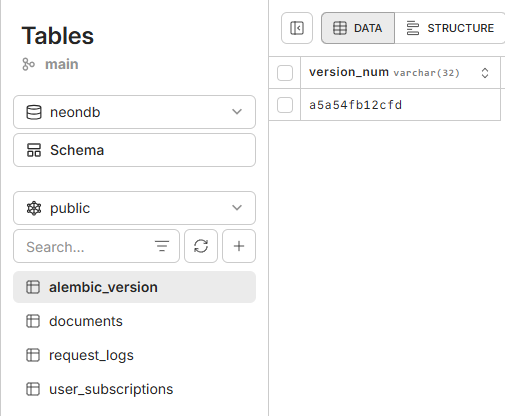
\includegraphics[width=0.6\textwidth]{pictures/document-database.png}
\caption{Kết quả các bảng trong CSDL tài liệu}
\end{figure}

%%%%%%%%%%%%%%%%%%%%%%%%%%%%%%%%%%%%%%
% Mô tả chi tiết thông tin bảng trong CSDL
%%%%%%%%%%%%%%%%%%%%%%%%%%%%%%%%%%%%%%
% thứ tự các bảng trong tài liệu

\begin{table}[H]
\centering
\begin{tabular}{|l|l|p{6cm}|}
\hline
\textbf{Cột} & \textbf{Kiểu dữ liệu} & \textbf{Mô tả} \\ \hline
version\_num & varchar & Mã phiên bản di chuyển CSDL. \\ \hline
\end{tabular}
\caption{Cấu trúc bảng \texttt{alembic\_version} (Dịch vụ văn bản)}
\end{table}

\begin{table}[H]
\centering
\begin{tabular}{|l|l|p{6cm}|}
\hline
\textbf{Cột} & \textbf{Kiểu dữ liệu} & \textbf{Mô tả} \\ \hline
id & uuid & Khóa chính của log yêu cầu HTTP. \\ \hline
request\_id & varchar & Mã định danh duy nhất của yêu cầu. \\ \hline
method & varchar & Phương thức HTTP được sử dụng. \\ \hline
url & varchar & Đường dẫn của yêu cầu API. \\ \hline
client\_ip & varchar & Địa chỉ IP của máy khách gửi yêu cầu. \\ \hline
status\_code & int4 & Mã trạng thái phản hồi HTTP trả về. \\ \hline
request\_payload & json & Dữ liệu chi tiết gửi kèm trong yêu cầu. \\ \hline
response\_payload & json & Dữ liệu chi tiết do hệ thống phản hồi. \\ \hline
process\_time & float8 & Thời gian xử lý hoàn tất yêu cầu. \\ \hline
created\_at & timestamptz & Thời gian ghi nhận log hệ thống. \\ \hline
\end{tabular}
\caption{Cấu trúc bảng \texttt{request\_logs} (Dịch vụ văn bản)}
\end{table}

\begin{table}[H]
\centering
\begin{tabular}{|l|l|p{6cm}|}
\hline
\textbf{Cột} & \textbf{Kiểu dữ liệu} & \textbf{Mô tả} \\ \hline
id & uuid & Khóa chính của bản ghi đồng bộ gói đăng ký người dùng. \\ \hline
user\_id & varchar & ID người dùng đồng bộ. \\ \hline
subscription\_id & varchar & Mã định danh gói thuê bao. \\ \hline
is\_active & bool & Cờ xác nhận trạng thái quyền VIP. \\ \hline
created\_at & timestamptz & Thời gian tạo bản ghi đồng bộ. \\ \hline
updated\_at & timestamptz & Thời gian cập nhật dữ liệu đồng bộ gói. \\ \hline
period\_start & timestamptz & Thời điểm bắt đầu có hiệu lực. \\ \hline
period\_end & timestamptz & Thời điểm kết thúc/hết hạn. \\ \hline
version & int4 & Phiên bản của bản ghi sự kiện, dùng để loại bỏ các sự kiện cũ (out-of-order). \\ \hline
\end{tabular}
\caption{Cấu trúc bảng \texttt{user\_subscriptions} (Dịch vụ văn bản)}
\end{table}

\begin{table}[H]
\centering
\begin{tabular}{|l|l|p{6cm}|}
\hline
\textbf{Cột} & \textbf{Kiểu dữ liệu} & \textbf{Mô tả} \\ \hline
id & uuid & Khóa chính định danh tài liệu. \\ \hline
user\_id & varchar & ID người dùng tạo và sở hữu tài liệu. \\ \hline
filename & varchar & Tên tệp tin khi người dùng tải lên. \\ \hline
status & varchar & Trạng thái xử lý tổng thể của tài liệu. \\ \hline
created\_at & timestamptz & Thời gian tài liệu được tạo. \\ \hline
updated\_at & timestamptz & Thời gian cập nhật tài liệu gần nhất. \\ \hline
has\_file & bool & Cờ xác nhận tệp gốc đã được tải lên. \\ \hline
has\_content & bool & Cờ xác nhận tài liệu đã được bóc tách nội dung (Markdown) thành công. \\ \hline
has\_summary & bool & Cờ xác nhận tài liệu được tóm tắt. \\ \hline
file\_hash & varchar & Mã băm của tệp tin, dùng để phát hiện và tái sử dụng tài liệu trùng lặp. \\ \hline
file\_size & int4 & Dung lượng của tệp tin, kết hợp với file\_hash để tái sử dụng. \\ \hline
\end{tabular}
\caption{Cấu trúc bảng \texttt{documents} (Dịch vụ văn bản)}
\end{table}
